\documentclass[9pt]{extarticle}

\usepackage[utf8]{inputenc}
\usepackage[T1]{fontenc}
\usepackage{lmodern}
\usepackage{graphicx}
\usepackage{color}
\usepackage{hyperref}
\usepackage{amsmath}
\usepackage{amsfonts}
\usepackage{epstopdf}
\usepackage[table]{xcolor}
\usepackage[a4paper, total={6in, 10in}]{geometry}
\usepackage{enumitem}
\usepackage[export]{adjustbox}


\graphicspath{ {./Figures/} }

\begin{document}

{\huge Andrew Sivaprakasam | Final Project - Progress Report 3}
\begin{center}
Final Project Repo: \url{https://github.com/sivaprakasaman/BME_511_FinalProject} \\
\end{center} 

\underline{Current State of the project:}\\ 

Decent progress, still a lot to do but starting to get going on finding the best way to analyze data. Main progress from last week includes getting modulation and carrier-frequency PSDs working for a given stimulus (see SAM tone and Violin stimuli below). I tried a few different PSD calculations. But it appears using multi-taper estimates are helpful because I can adjust the time-bandwidth product to focus in on spectral features I'm interested in.

Before the presentation, I'm trying to get a good measure of the correlation between the apPSTH Modulation/Carrier Frequency (ENV/TFS respectively) spectrum and that of the stimulus ENV and TFS. After meeting with Satya, it appears a good way to do this is first passing the stimulus through a filter bank to get spectra that correspond to a particular CF, rather than the whole-band stimulus. This would result in a more realistic analysis since the apPSTHs generated correspond to a particular CF, rather than a wide-band filter. 

After passing the stimulus through a filterbank (I'm planning on using 125 Hz, 440 Hz ($F_0$), 880 Hz ($F_1$), and 4 kHz as my CFs) and extracting Hilbert TFS/ENV I'll plan to get a magnitude-squared coherence spectrum to demonstrate the coding strength of timbral features (i.e. harmonics, envelope). We can then observe if this coding strength is consistent across instruments/articulations and if it's impacted by hearing loss.\\ 

\textbf{Figures:}\\

\centering
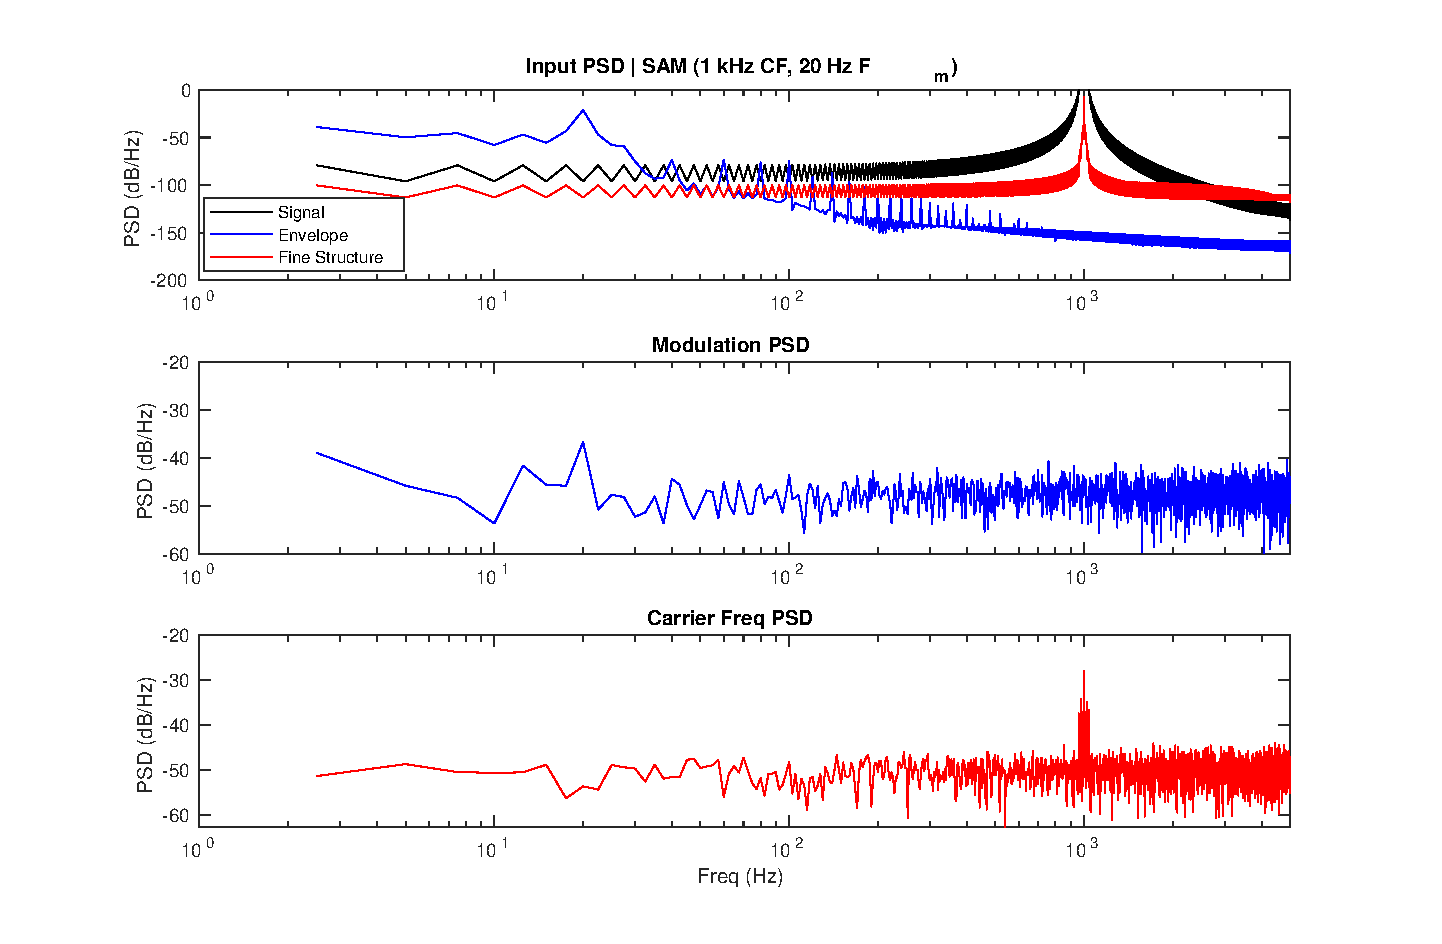
\includegraphics[width = .7\textwidth]{SAM_PSD}
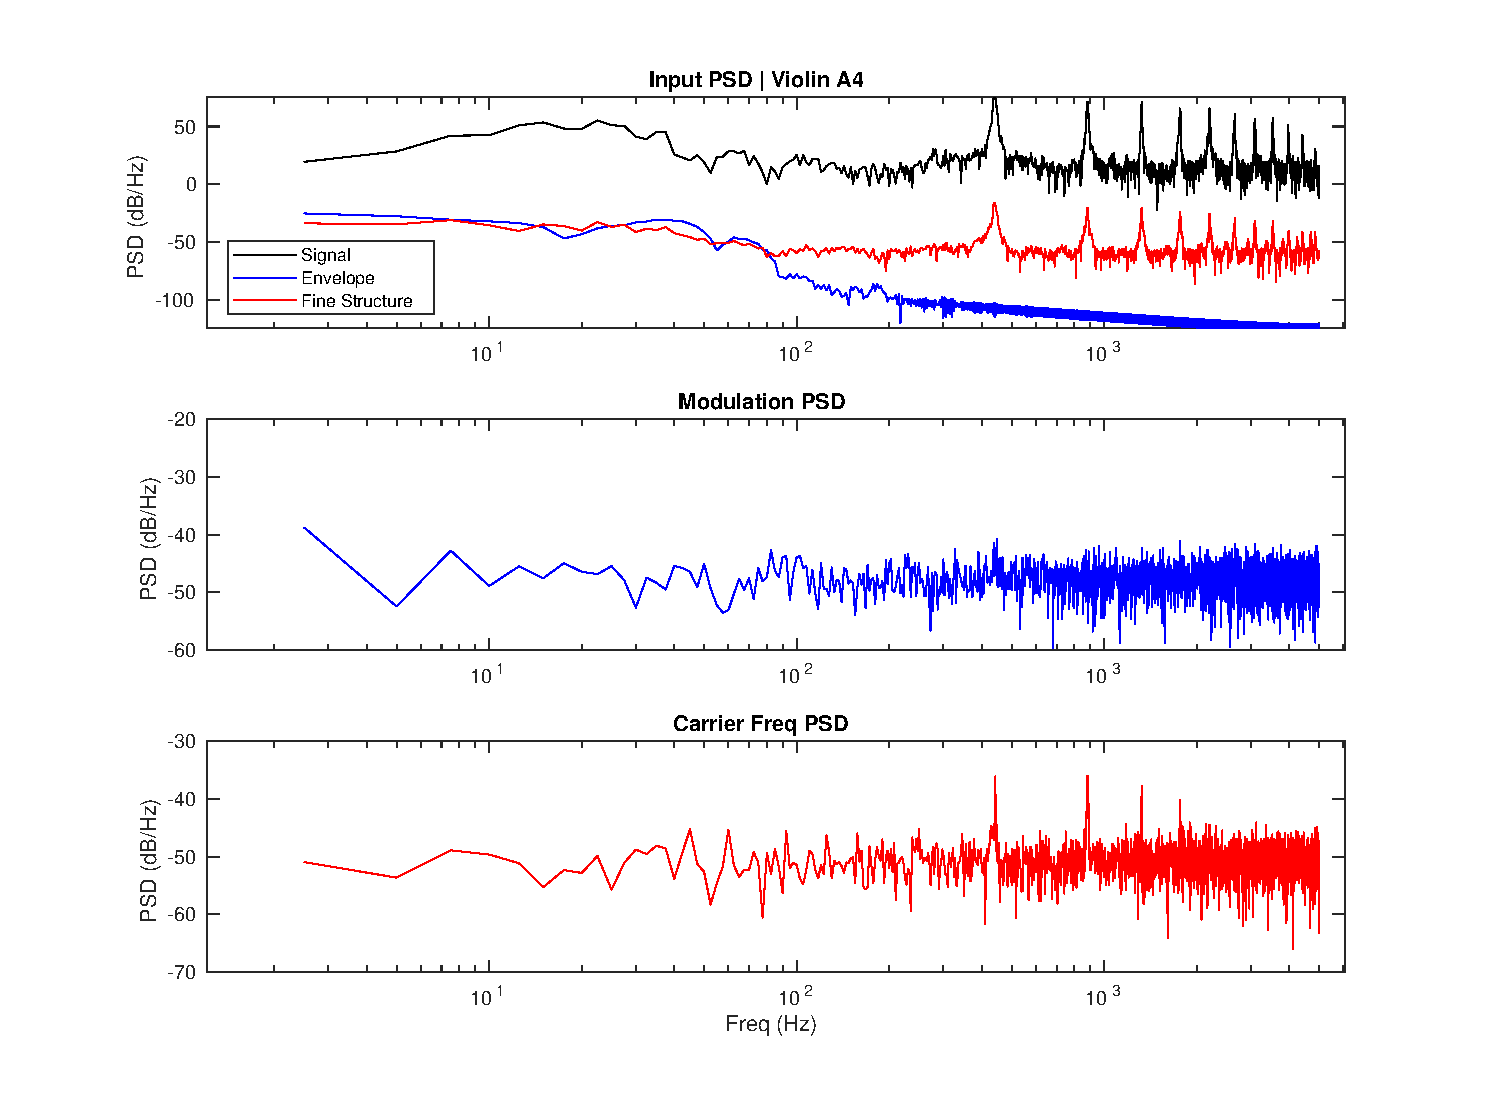
\includegraphics[width = .7\textwidth]{Violin_PSD}




\end{document}
